
%\begin{figure}[ht!]
%%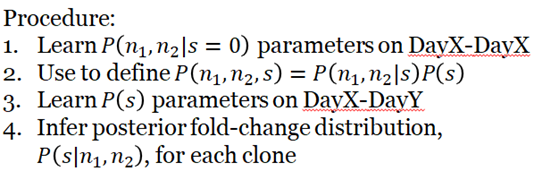
\includegraphics{procedure.png}
%%centering{}
%\caption{
%\emph{Supp. Fig: \re{What to show here?}Approximate equivalence of $N\langle f \rangle=1$ and $\mathcal{Z}^{\mathcal{D}}_f$.\label{fig:SM_match_null_constr}}}
%\end{figure}

\begin{figure}
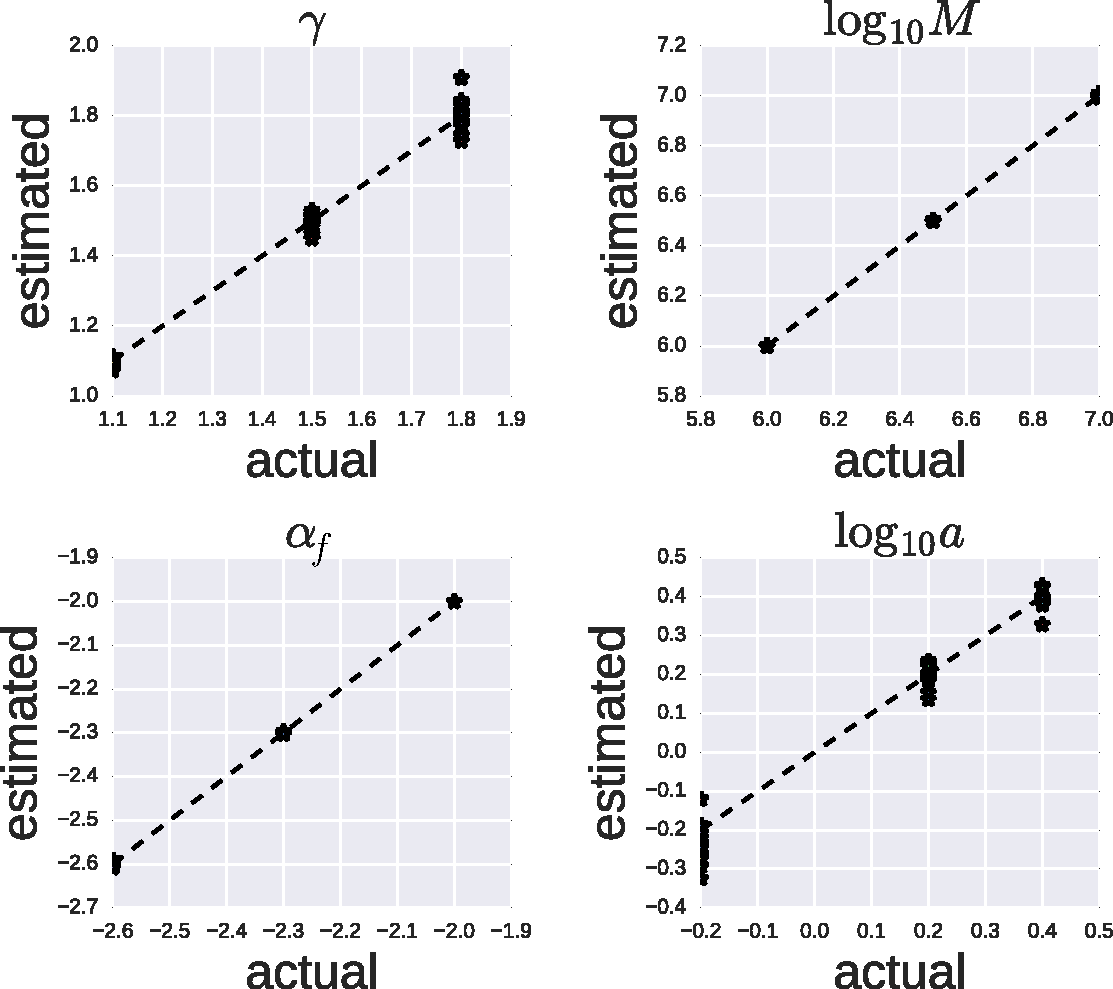
\includegraphics[width=\linewidth]{NB_Pois_nullpara_fits}
\centering{}
\caption{
\emph{Reinferring null model parameters}. Shown are the actual and estimated values of the null model parameters used to validate the null model inference procedure over the range exhibited by the data. A 3x3x3x3 grid of points were sampled and results collapsed over each parameter axis. $f_{\rm min}$ was fixed to satisfy the normalization constraint.
}
\label{fig:SM_reinfer_null}
\end{figure}

\begin{figure}
\includegraphics[width=\linewidth]{conditional_comparison}
\centering{}
\caption{
\emph{Dependence of conditional distribution $P(n^\prime=0|n)$ on $n$}. Two-step negative binomial to Poisson model captures tail better than one-step negative binomial model. Poisson model fits poorly. (Example donor S2-day 0 replicate pair.)\label{fig:SM_twostep_better}
}
\end{figure}



\begin{figure}
\includegraphics[width=\linewidth]{synthetic_reinference}
\centering{}
\caption{
\emph{Reinference of differential expression model for human-sized repertoire}. $10^9$ clones were sampled using $N_{\rm read}=10^6$ and $(\bar{s},\alpha)=(1.0,0.01)$ (cross), and clones with $n=n^\prime=0$ were removed. Note the orders of magnitude higher precision compared to the synthetic mouse repertoire \cref{fig:diffexpr_ex1}. 
\label{fig:SM_reinf_diffexpr}}
\end{figure}

\begin{figure}
\includegraphics[width=\linewidth]{s_naive_hist}
\centering{}
\caption{
\emph{Empirical histograms of naive log-frequency fold-change}. For example data: day-0/day-0 and day-0/day-15 pair comparisons averaged over donors.
\label{fig:SM_snaive_hists}
}
\end{figure}

\begin{figure}
\includegraphics[width=\linewidth]{s_med_vs_snaive}
\centering{}
\caption{
\emph{Summary statistics of log-frequency fold-change posterior distributions}. Comparison of the posterior median log-frequency fold-change and the naive estimate, $\log n^{\prime}/n$ (across clones with $n,n^{\prime}>0$). Each circle is a $(n,n^\prime)$ pair with size proportional to pair count average $(n+n^\prime)/2$ and intensity proportional to the number of observed clones with that pair.
\label{fig:SM_smed_snaive}
}
\end{figure}

\begin{figure}
\includegraphics[width=\linewidth]{posterior_ridge_sweep}

%\centering{}
\caption{
\emph{Competition between $\nu$ and $\bar{s}$ in shaping the posteriors, $\rho(s|0,n^\prime)$}. A) Posteriors for $n^\prime=9$ over a range of $(\bar{s},\alpha)$ pairs spanning the ridge shown in the inset in (B) and \cref{fig:volcano} along which the growth of $\bar{s}$ leads to $\rho(f)$ overwhelming $\rho_s(s)$ as the dominant explanation for observed expansion. (B) The posterior mean versus $\bar{s}$ for values of $n^\prime=1,\dots,9$, with the 5 values of $\bar{s}$ used in (A) shown for $n^\prime=9$.
\label{fig:posteriors}}
\end{figure}